\section{Aufbau und Durchführung}
\label{sec:Durchführung}
In diesem Abschnitt wird zunächst der Aufbau und die Einstellung der verwendeten Messapparatur beschrieben und anschließend die Durchführung des Experimentes dokumentier.
\subsection{Aufbau der Messapparatur}
\label{sec:aufbau}
Die verwendete Messapparatur ist in Abbildung \ref{fig:messapp} zu sehen.
\begin{figure}[h]
  \centering
  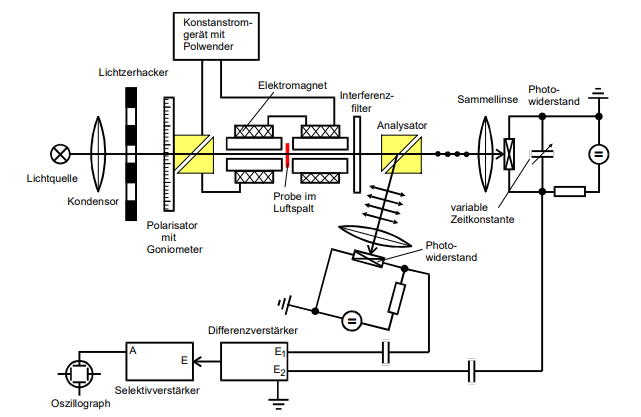
\includegraphics[scale=0.5]{fig/messapp.png}
  \caption{Der schematische Aufbau des Versuches. \cite[2]{Anleitung2}}
  \label{fig:messapp}
\end{figure}
In diesem Experiment dient eine Halogenlampe mit Emissionsspektrum im Infrarotbereich als Lichtquelle. Das dort emittierte Licht gelangt mit Hilfe einer Kondensorlinse parallel in den nächsten Teil des Aufbaus. Von einem Lichtzerhacker aus wird das gesammelte Licht in ein aus Kalkspat bestehendes Glan-Thompson-Prisma (siehe Abbildung \ref{fig:glan}) weitergeleitet.
\begin{figure}[h!]
  \centering
  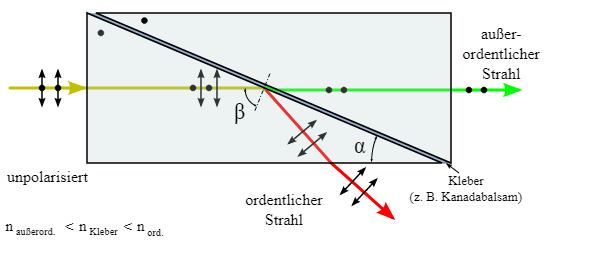
\includegraphics[scale=0.5]{fig/glan.png}
  \caption{Der schematische Aufbau eines Glan-Thompson-Prisma. \cite{Anleitung3}}
  \label{fig:glan}
\end{figure}
In diesem wird das linear polarisierte Licht erzeugt, das in diesem Versuch untersucht werden soll.\\ Die zu untersuchende Probe befindet sich in einem Magnetfeld, das von einem Elektromagneten erzeugt wird.
Dabei ist es notwendig, dass, wie in
\ref{sec:Theorie} beschrieben, der Magnetfeldvektor parallel zum Vektor der einfallenden Lichtwelle ist. Das Magnetfeld wird dabei von einem Konstantstrom gerät gespeist, damit es zeitlich konstant ist. Sobald die Welle aus der Probe austritt wird das Wellenlängenspektrum mit Hilfe eines Interferenzfilters (siehe Abbildung \ref{fig:inter}) auf eine Wellenlänge reduziert und trifft anschließend auf das zweite Glan-Thompson-Prisma.
\begin{figure}[h!]
  \centering
  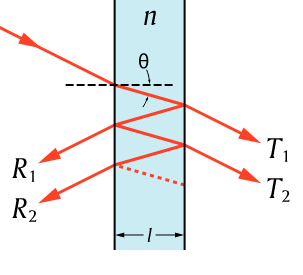
\includegraphics[scale=0.5]{fig/inter.png}
  \caption{Der schematische Aufbau eines Interferenzfilters. \cite{Anleitung4}}
  \label{fig:inter}
\end{figure}
Über die Schichtdicke des Dielektrikums des Interferenzfilter wird die transmittierte Wellenlänge festgelegt. Aus dem zweiten Glan-Thompson-Prisma treten nun zwei Strahlenbündel aus, deren
Intensität von der Polarisation des eingehenden Lichtstrahls abhängt und die orthogonal zueinander polarisiert sind, dies dient einer hohen Winkelauflösung.\\
Anschließend werden diese jeweils mit einer Sammellinse gebündelt und mit Hilfe einer Photodiode wird die Intensität des Lichtes in einen Strom ungewandelt. Dieses Signal wird an die beiden Eingänge eines
Differenzverstärkers angeschlossen und dieser liefert einer zur Differenz der Eingangsspannungen proportionale Ausgangsspannung. Der daran angeschlossene Selektivverstärker wird auf die Frequenz des Lichtzerhackers eingestellt um
das entstehende Rauschen deutlich zu verringern. Als letztes wird auf einem Oszilloskop das endgültige Signal sichtbar gemacht.
\subsection{Durchführung}
\label{sec:durch}
Vor der Messung wird zunächst die Messapparatur kalibriert, das bedeutet es wird überprüft ob die Sammellinse die Strahlen vernünftig auf die Photodioden leitet. Um den Selektivverstärker einzustellen wird dieser auf die Frequenz
des Lichtzerhackers eingestellt. Anschließend wird das Signal einer Photodiode auf die Licht fällt auf den "Input" des Selektivverstärkers gegeben und das Oszilloskop wird an den Augang "Resonance" angecschlossen. Nun wird mit Hilfe der
Frequenzstellknöpfe am Selektivverstärker solange justiert bis sich ein maximales Ausgangssignal ergibt, das heißt die Signalamplitude auf dem Oszilloskop maximal gro0 ist. \\
Das Magnetfeld im Inneren der Spule wird mit einer Hallsonde vermessen, um den Ort des maximalen Magnetfeldes zu bestimmen. \\
Jetzt beginnt die Messung um den Polarisationswinkel $\vartheta$ zu bestimmen, dafür wird das Goniometer am ersten Glan-Thompson-Prisma verwendet.
 Eine Probe sowie Interferenzfilter werden eingesetzt und das Goniometer wird anschließend variiert bis das Signal am Oszilloskop minimal wird.
  Dann wird der erste Polarisationswinkel $\vartheta_\mathrm{1}$ notiert und das Magnetfeld wird mit Hilfe des Konstantstromgerätes umgepolt. Dann wird der Vorgang wiederholt und der zweite
Polarisationswinkel $\vartheta_\mathrm{2}$ wird notiert. Der Drehwinkel der Polarisationsebene lässt sich über den folgenden Zusammenhang berechnen:
\begin{equation}
  \label{eqn:rotawinkel}
  \vartheta=\dfrac{1}{2}(\vartheta_\mathrm{1}-\vartheta_\mathrm{2})
\end{equation}
Man wiederholt die Messungen nun mit verschiedenen Interferenzfiltern und den daraus resultierenden unterschiedlich gefilterten Wellenlängen.
